\documentclass[border=4pt]{standalone}
\usepackage{tikz}
\usetikzlibrary{arrows.meta,positioning,shapes.geometric}
\begin{document}
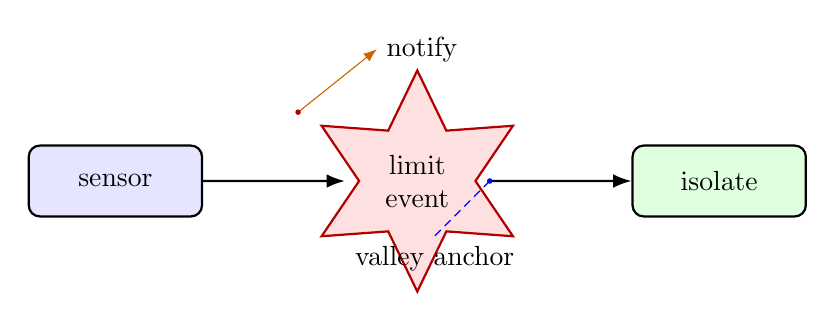
\begin{tikzpicture}[
  >=Latex,
  node distance=18mm,
  process/.style={draw,thick,rounded corners,minimum width=22mm,minimum height=9mm},
  event/.style={star,star points=6,star point ratio=1.9,draw=red!70!black,
    thick,fill=red!12,minimum size=17mm,outer sep=1.5mm,align=center}
]
  \node[process,fill=blue!10] (sensor) {sensor};
  \node[event,right=of sensor] (alarm) {limit\\event};
  \node[process,fill=green!12,right=of alarm] (isolate) {isolate};

  \draw[-Latex,thick] (sensor) -- (alarm);
  \draw[-Latex,thick] (alarm) -- (isolate);
  \draw[-Latex,orange!80!black] (alarm.outer point 2) -- ++(10mm,8mm)
    node[right,black] {notify};
  \draw[densely dashed,blue] (alarm.inner point 5) -- ++(-7mm,-7mm)
    node[below,black] {valley anchor};
  \fill[red!70!black] (alarm.outer point 2) circle (1pt);
  \fill[blue] (alarm.inner point 5) circle (1pt);
\end{tikzpicture}
\end{document}
